\documentclass[
	fullscreen=true, 
	bookmarks=false,
	sans serif,
	9pt,
	pdf,
	hyperref={
		pdfpagelabels=false,
		unicode=true
	}
]{beamer}
\usepackage[T2A]{fontenc}
\usepackage[utf8]{inputenc}
\usepackage[english,russian]{babel}
\usepackage{pgfpages}
\pgfpagesuselayout{resize to}[a4paper,landscape,border shrink=0mm]

\usepackage{array}
\usepackage{epsfig}
\usepackage{epstopdf}
\usepackage{multirow}
\usepackage{listings}
\usepackage{tikz}

\lstset{
	tabsize=4,
	gobble=12,
	keepspaces=true,
	basicstyle=\normalsize\ttfamily,
	breaklines=true,
	columns=fullflexible,
}

\usetheme{Madrid}
% =====================================================================

% Info
\title{
	Модель прогнозирования успеваемости студентов на основе демографическичх и социально-экономических показателей
}
\author{
	\vspace{0.5cm}\\
	\large
    Шупинский В. А.\\
	\vspace{0.1cm}
	УлГТУ\\
	\vspace{2cm}
}
\institute{}
\date{08.12.2021}
% =====================================================================

% Document
\begin{document}
	
	% Title
	\begin{frame}
		\titlepage
	\end{frame}	
	% =====================================================================
		
	\section{}
	\subsection{}
		
	\begin{frame}\frametitle{Цель}
		– Обратить внимание преподавателя на обучающихся, которые могут иметь пониженную успеваемость, путём прогноза до начала обучения. Это поможет уменьшить кол-во учеников, которые будучи обделёнными вниманием преподавателя перестали учиться.
		\newline
		
		Данные:
		\begin{enumerate}
			\item Пол
			\item Этнос
			\item Образование родителей
			\item Обед
			\item Подготовительные курсы
		\end{enumerate}
		Данные для создания модели:
		\begin{enumerate}
			\item Балл математики
			\item Балл русского
			\item Балл предмета по выбору 
		\end{enumerate}
	\end{frame}

	\begin{frame}\frametitle{Задачи и методы}
		Задача лишь одна, обеспечить представление преподавателя о его учениках до начала работы с ними.
		\newline
		
		Методы:
		\begin{itemize}
			\item k-средних Мак-Кина;
			\item Кластеризация группа объединённых по результатам из обучающей выборки;
			\item Предположение на основе выделенных групп и коррелции.
		\end{itemize}
	\end{frame}

	\begin{frame}\frametitle{Научная новизна}
		Существуют системы прогноза на оценках или других четких шкалах. Способы же предсказания успеваемости есть только в исследованиях, но нет реальных систем.
		\begin{figure}
			\centering
			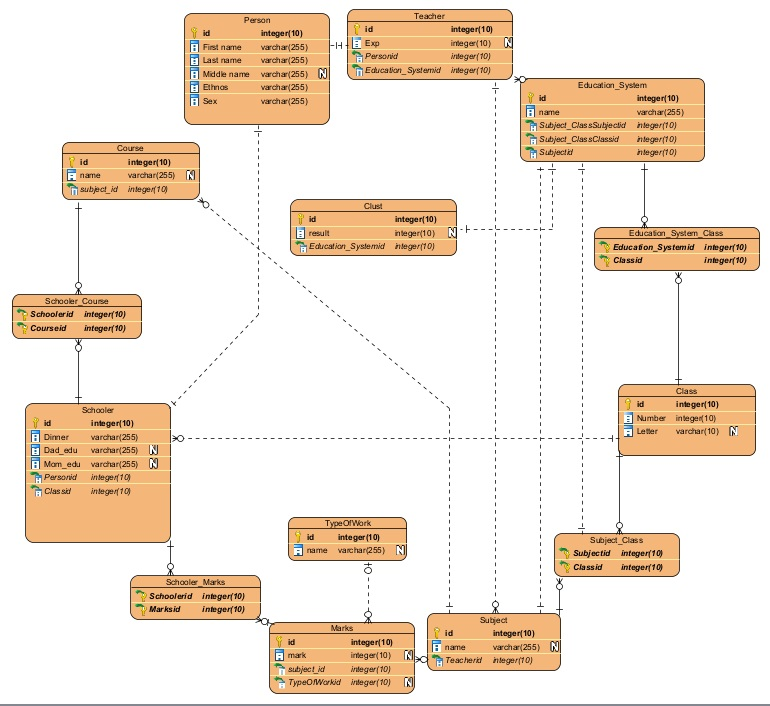
\includegraphics[width=0.5\linewidth]{images/student}
		\end{figure}
	\end{frame}

	\begin{frame}\frametitle{Краткий обзор научных работ по тематике}
		\begin{tabular}{|p{2cm}|p{4.3cm}|p{4.3cm}|}
			\hline 
			Ерофина Е.А. и Хруслова Д.В  & О некоторых зависимостях успеваемости студентов & Успеваемость напрямую зависит от понимания своей деятельности группой, хорошего расписания и наличия свободного времени \\ 
			\hline 
			Кузнецов В.В., Байрамов Р.А., Смирнов Е.А., Косилова Е.К., Косилов К.В. & Взаимосвязь самооценки состояния здоровья и уровня заболеваемости с академической успеваемостью у студентов старших курсов медицинских специальностей с учетом влияния социально-экономических и демографических характеристик & Чем удобнее расписание человека подогнано под его ритм жизни, тем эффективнее он сможет работать и успешнее будет \\ 
			\hline 
		\end{tabular}		
	\end{frame}

	\begin{frame}\frametitle{Краткий обзор научных работ по тематике}
		\begin{tabular}{|p{2cm}|p{3.3cm}|p{5.3cm}|}
			\hline 
			Шухмана А.Е., Парфенова Д.И., Легашева Л.В и Гришиной Л.С. & Анализ и прогнозирование успеваемости обучающихся при помощи использование цифровой образовательной среды  & Студенты не показали динамики результатов с переходом на дистанционное обучение, но процент сдающих вовремя заметно снизился. Прогноз успеваемости обучающихся опирался на внешние факторы: возраст, пол, состояние здоровья, результаты вступительных экзаменов, внеучебная деятельность студентов, временная или постоянная работы, участие в мероприятиях \\ 
			\hline 
			Шевченко В.А & Прогнозирование успеваемости студентов на основе методов кластерного анализа & Метод k-средних Мак-Кина, модифицированный под нужды задачи прогнозирования успеваемости \\ 
			\hline 
			Зяблецева Павла Андреевича & Прогнозная модель для оценки успеваемости студентов университета по итогам текущего обучения & Описана возможная модель прогнозирования успеваемости \\ 
			\hline 
		\end{tabular}		
	\end{frame}
	
	\begin{frame}\frametitle{Положения вносимые в защиту}
		Основываясь на образовании родителей, их философии а также заробатке вполне можно предположить, какими они воспитают детей, а уже на этом можно строить прогноз успеваемости этих детей.
	\end{frame}

	\begin{frame}\frametitle{}
		\Large
		\center
		\textbf{Спасибо!}\\
		\vspace{1.5cm}
		\normalsize
		Шупинский В.А.\\
		Подразделение\\
		УлГТУ\\
		\vspace{0.5cm}
		\textit{ContractWithDevil@yandex.ru}
	\end{frame}
	
\end{document}
